% Exercise ID: MAT_P4FUNCOE_0PX_IGX_002
% Created: 2025-11-26
% Difficulty: 2/5

\exercicio{
No plano cartesiano está desenhado o seguinte retângulo:

\begin{center}
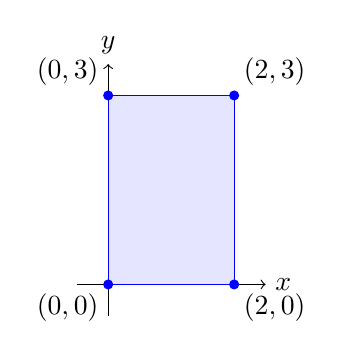
\begin{tikzpicture}[scale=0.8]
    % Eixos
    \draw[->] (-0.5,0) -- (2.5,0) node[right] {$x$};
    \draw[->] (0,-0.5) -- (0,3.5) node[above] {$y$};
    % Retângulo
    \draw[fill=blue!10,draw=blue] (0,0) rectangle (2,3);
    % Vértices
    \foreach \x/\y in {0/0, 0/3, 2/0, 2/3}
        \filldraw[blue] (\x,\y) circle (2pt);
    % Coordenadas dos vértices
    \node[below left] at (0,0) {$(0,0)$};
    \node[above left] at (0,3) {$(0,3)$};
    \node[below right] at (2,0) {$(2,0)$};
    \node[above right] at (2,3) {$(2,3)$};
\end{tikzpicture}
\end{center}

Indique o produto cartesiano de intervalos que corresponde ao conjunto de pontos do retângulo.
}
